\section{PID Tunning}\label{sec:PID_Tunning}

With a view to ensure a tracking communication between the Drone and its ground station, and thus, keep a proper angle of the directions of the antennas, a controller has been designed.\par

The actuator to be controlled is a servo motor having the desired characteristics for this application.  Reaching speed, accuracy and weight of the antenna were taken into account to determine the appropriate motor. Based on the above mentioned, a PID controller was chosen to perform this task. (WHY PID ?) (explanation of P I and D?)\par

Can be seen on the figure below, the structure of the controller. Taking as input the error angle \textbf{$\phi_{e}$} and outputting the necessary voltage \textit{Vm} for the motor, this controller has the final task of converting a value in radian into voltage.\par

\begin{figure}[H]
  \centering
  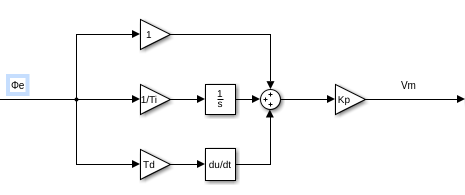
\includegraphics[scale=0.5]{figures/PID_2D.png}
  \caption[LABEL] {Block diagram of the PID controller}
\end{figure}
  
Different methods can be used to tune a PID controller as the, Zieggler-Nichols, Skogestad and Good Gain method, having in common the same goal : Get a fast response and provide a good stability. The Good Gain is the method that has been chosen in our application to determine the parameters of the controller.\par
  
The steps of the experiment based method, the Good Gain, are the followings :\par 
  
\begin{itemize}
  \item Set Ti = inf , Td = 0 and Kp = 1
\end{itemize}
  
  \begin{figure}[H]
    \centering
    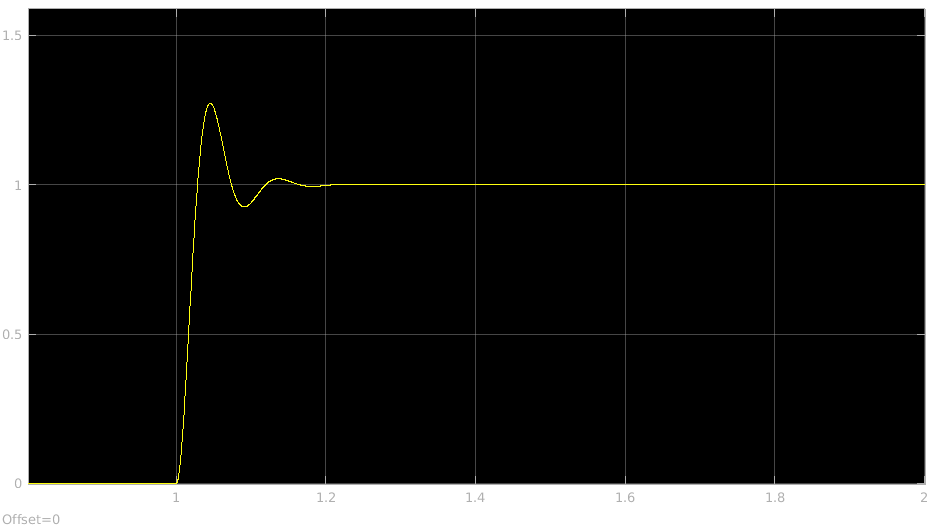
\includegraphics[scale=0.4]{figures/GoodGain_step1.png}
    \caption[LABEL] {Step response Good Gain method : stage 1} 
  \end{figure}
  

\begin{itemize}
  \item Increase or decrease Kp until finding a slight overshoot but a well damped response
\end{itemize}
  
  \begin{figure}[H]
    \centering
    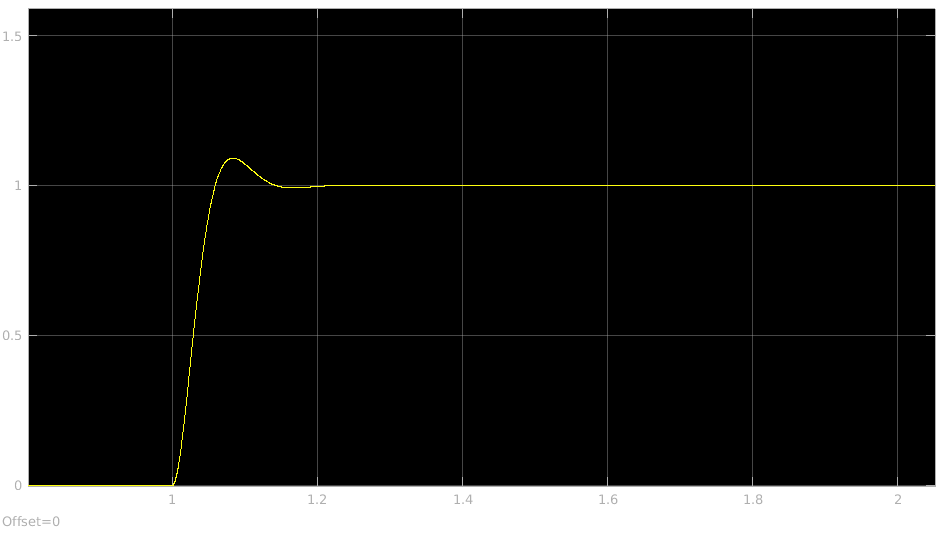
\includegraphics[scale=0.4]{figures/GoodGain_step2.png}
    \caption[LABEL] {Step response Good Gain method : stage 2} 
  \end{figure}
    
    
\begin{itemize}
  \item Set Ti = 1.5$\cdot T_{out}$
\end{itemize}
  
  \begin{figure}[H]
    \centering
    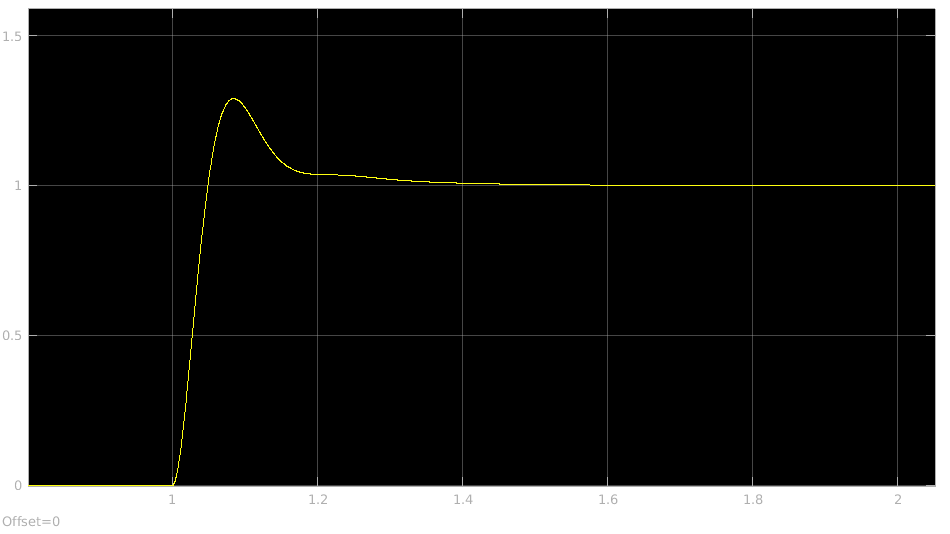
\includegraphics[scale=0.4]{figures/GoodGain_step3.png}
    \caption[LABEL] {Step response Good Gain method : stage 3} 
  \end{figure}
    
    
\begin{itemize}
  \item Set Td = $\frac{Ti}{4}$
\end{itemize}
  
  \begin{figure}[H]
    \centering
    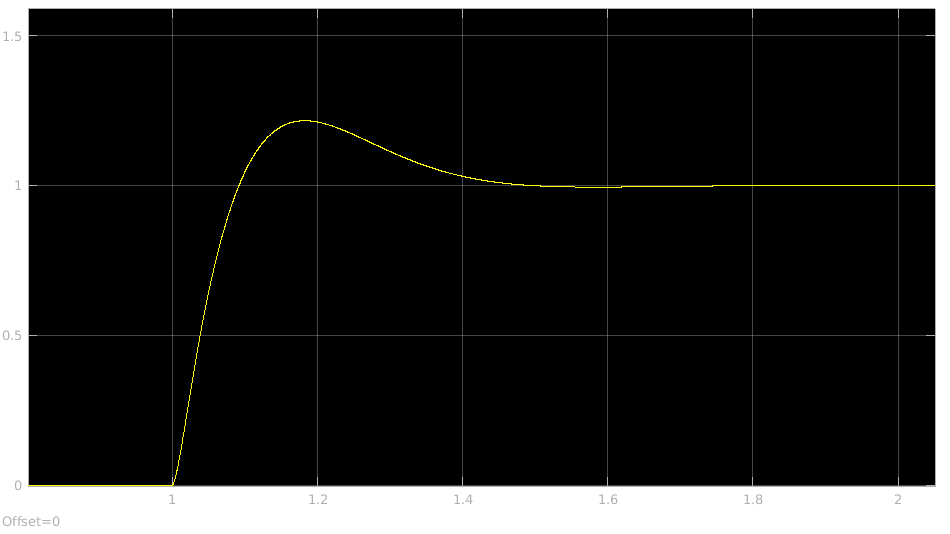
\includegraphics[scale=0.4]{figures/GoodGain_step4.png}
    \caption[LABEL] {Step response Good Gain method : stage 4} 
  \end{figure}